\documentclass[a4paper,12pt]{article}

\usepackage[utf8]{inputenc}
\usepackage{parskip}
\usepackage[ngerman]{babel}
\usepackage{graphicx}

\title{OOAD Übungsblatt 3}
\author{Dominik Tödling, Lukas Neuhold, Christoph Huber,\\ Stefan Mitterrutzner, Emanuel Moser}

\begin{document}
\maketitle
\newpage
\part*{Abgabe 1}
\subsection*{Sequence Diagram}
\begin{center}
	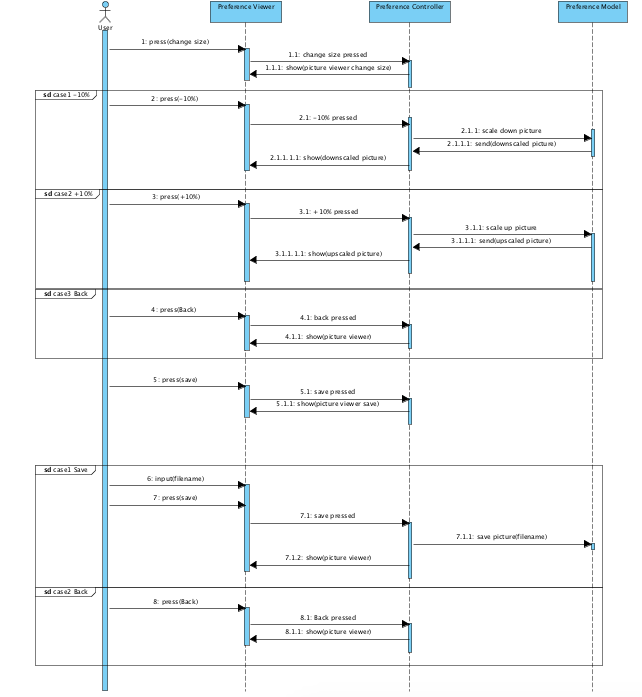
\includegraphics[scale=.6]{SequencePictureViewer.png}
\end{center}
\subsection*{Communication Diagram}
\begin{center}
	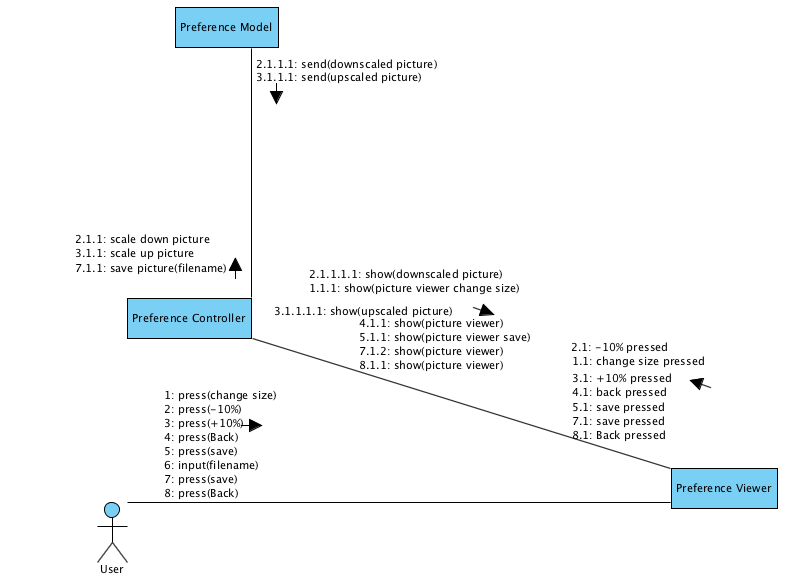
\includegraphics[scale=.6]{CommunicationsPictureViewer.png}
\end{center}
\subsection*{State Machine Diagram}
\begin{center}
	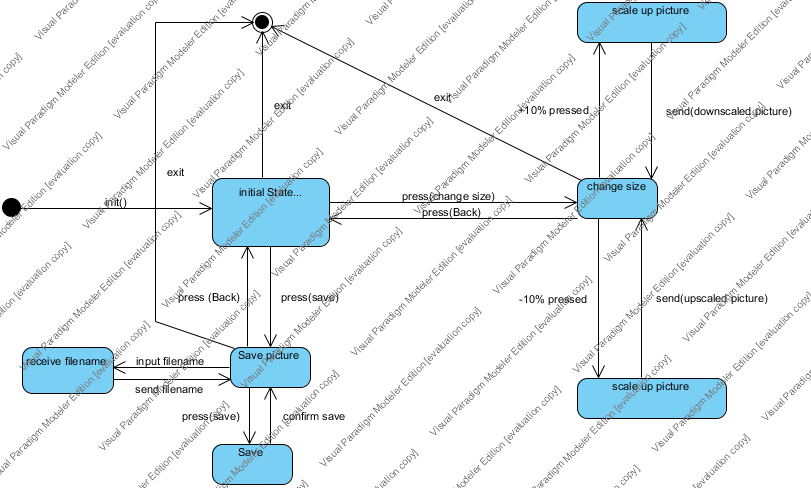
\includegraphics[scale=.6]{StatePictureViewer.png}
\end{center}
\newpage
\part*{Abgabe 2}
\section*{Business Case}
IntelliCourse ist eine Software zur Zeitplanung von Kursen. Durch die automatische Zeitplanerstellung kann sich jeder ganz einfach seinen eigenen Zeitplan einsehen. Ein jeder User kann einen individualisierten Kalender mit allen Terminen ganz einfach einsehen.  Beim erstellen eines Events wird automatisch auf Zeit- und Raumüberschneidungen überprüft, und gegebenenfalls ein Warning ausgegeben, und es wird automatisch versucht alles so anzupassen, dass es zu keiner Überschneidung kommt. Durch diese automatisierte Einteilung von Terminen auf mögliche Räume und Timeslots wird sich viel an administrativem Aufwand erspart, was ermöglicht die Kosten in der Administration zu senken.Zusätzlich ist es möglich das  LehrendeZeitpräferenzen einzugeben, die in die Erstellung des Zeitplans miteinbezogen werden. Im falle dass ein Termin zu einem bestimmten Zeitpunkt stattfinden MUSS, kann ein Administrator den Zeitplan immer manuel bearbeiten.
\section*{Use Cases}
	\subsection*{Priorisierung und Szenarien}
	\begin{tabular}{|p{3cm}|c|p{3cm}|c|p{3cm}|c|}
		\hline
		\textbf{Student} & \textbf{Score} & \textbf{Lehrender} & \textbf{Score} & \textbf{Admin} & \textbf{Score} \\ \hline
		Anmelden & 10 & Anmelden & 10 & Anmelden & 10 \\ \hline
		Für Veranstaltung registrieren & 10 & Für Veranstaltung registrieren & 10 & Account erstellen & 10 \\ \hline
		Account erstellen & 10 & Account erstellen & 10 & Accounts authorisieren & 10 \\ \hline
		Kalender einsehen & 9 & Veranstaltung erstellen & 10 & Zeitpräferenzen eingeben & 8 \\ \hline
		Event erstellen & 3 & Kurs erstellen & 10 & Zeitplan verändern & 7 \\ \hline
		&& Kalender einsehen & 9 & Zeitplan überprüfen & 7 \\ \hline
		&& Prüfung erstellen & 9 & Veranstaltung erstellen & 5 \\ \hline
		&& Zeitpräferenzen eingeben & 8 & Kurs erstellen & 4 \\ \hline
		&& Event erstellen & 3 & Prüfung erstellen & 4 \\ \hline
		&&&& Für Veranstaltung registrieren & 3 \\ \hline
		&&&& Kalender einsehen & 3 \\ \hline
		&&&& Event erstellen & 3 \\ \hline
		&&&& Raum erstellen & 10 \\ \hline
	\end{tabular}
	\newpage
	\subsection*{Use Case Spezifizierung}
	\begin{center}
		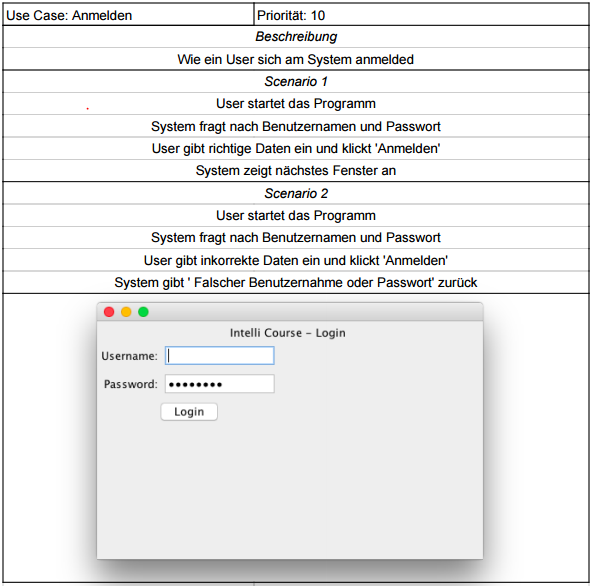
\includegraphics[scale=.8]{UCLogin.png}
		\newpage
		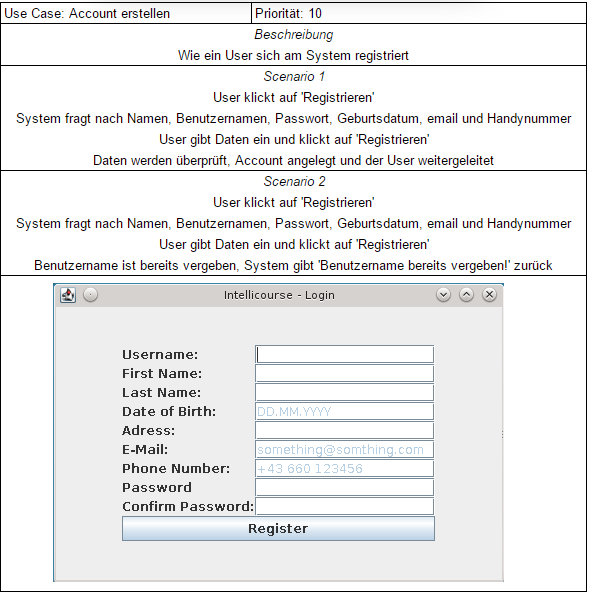
\includegraphics[scale=.8]{UCRegister.png}
		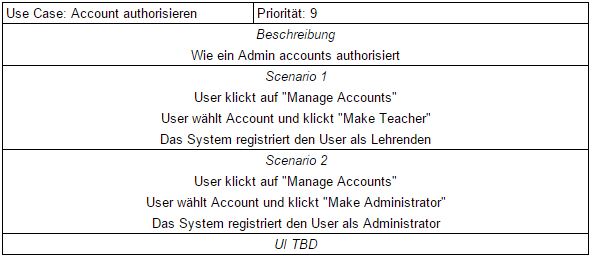
\includegraphics[scale=.8]{UCAuthorizeAccount.png}
		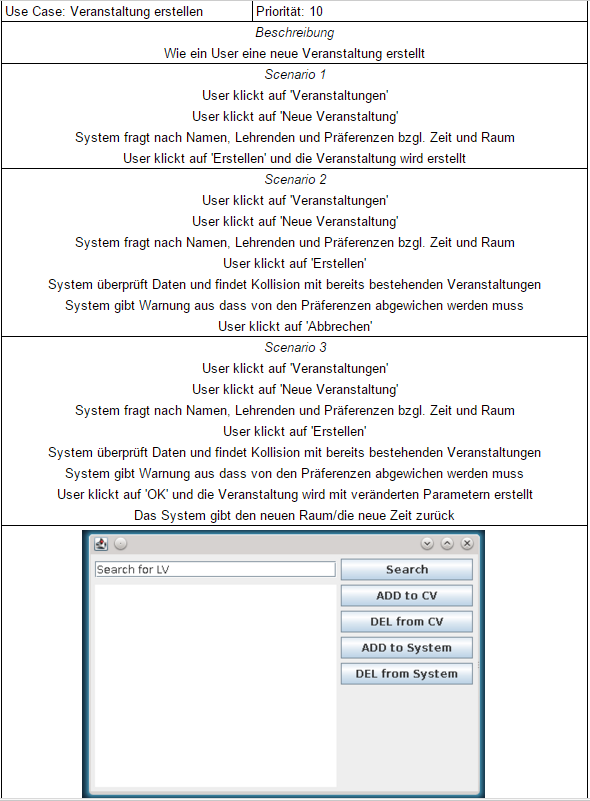
\includegraphics[scale=.8]{UCCreateHappening.png}
		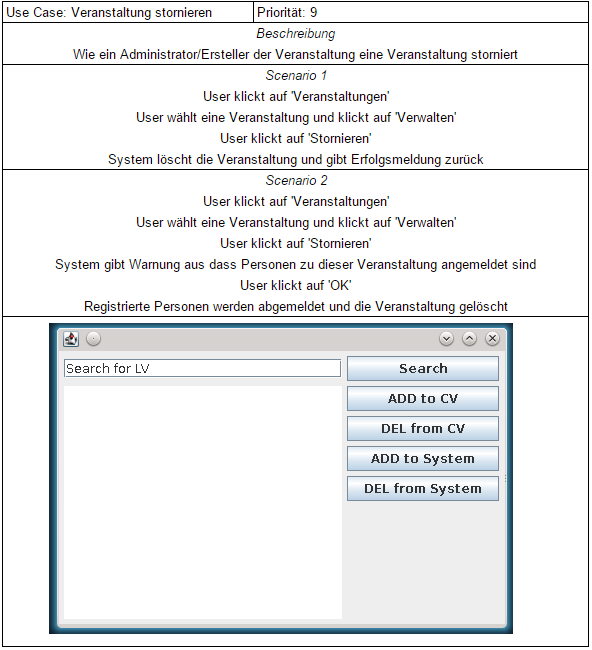
\includegraphics[scale=.8]{UCCancelHappening.png}
		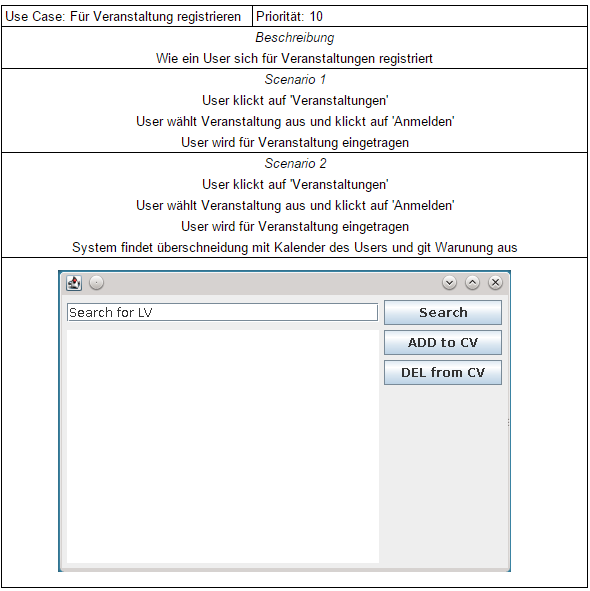
\includegraphics[scale=.8]{UCRegisterForHappening.png}
		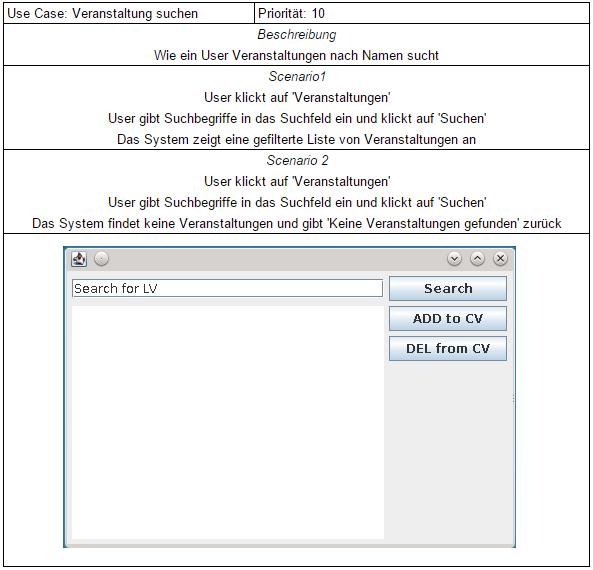
\includegraphics[scale=.8]{UCSearchHappening.png}
		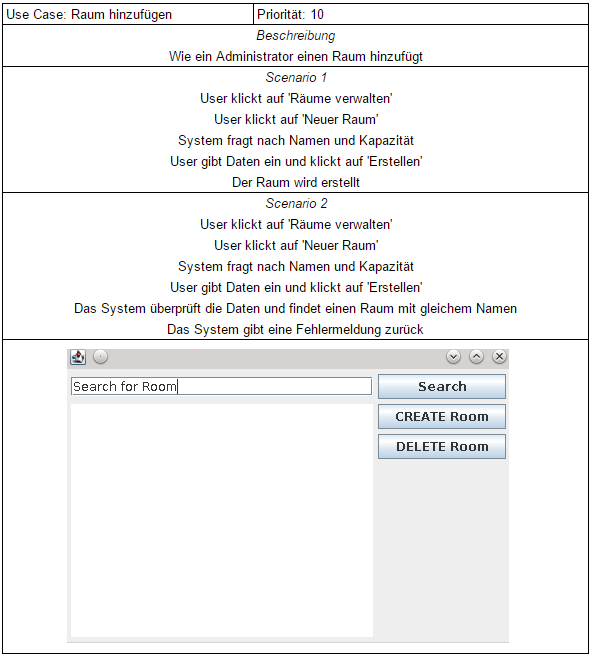
\includegraphics[scale=.8]{UCCreateRoom.png}
		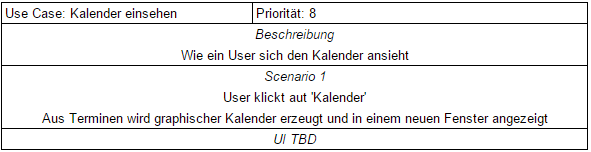
\includegraphics[scale=.8]{UCCalendar.png}
	\end{center}
	\subsection*{Use Case Diagramm}
	\begin{center}
		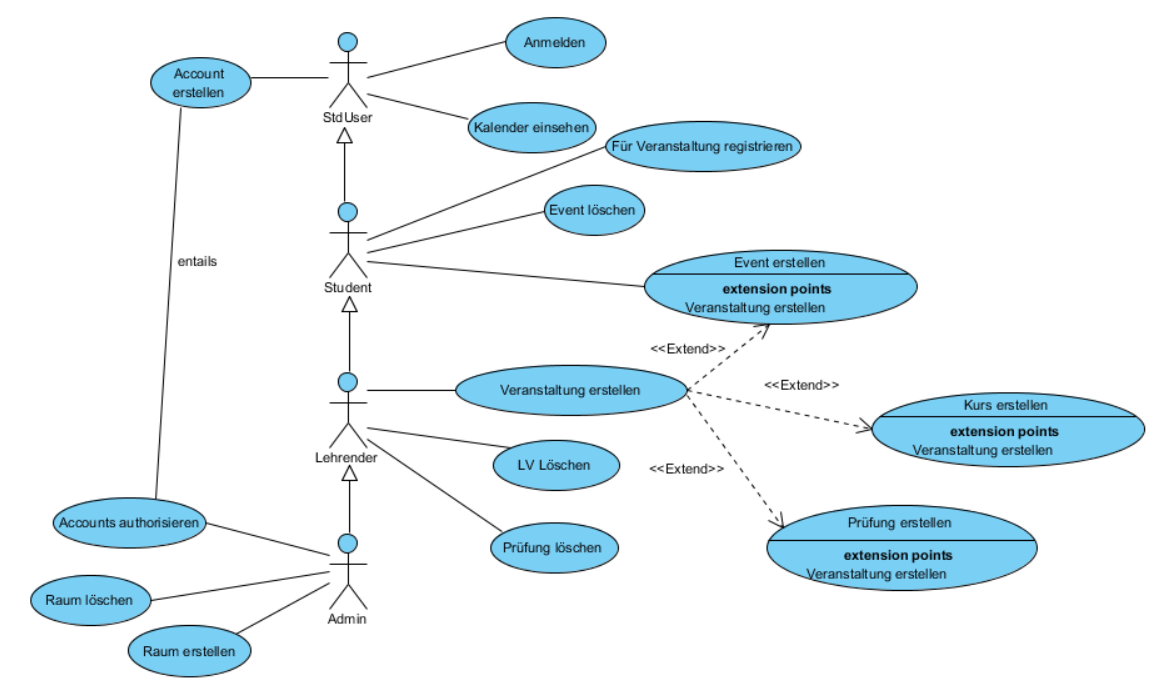
\includegraphics[scale=.5,angle=90]{UseCaseDiagram.png}
	\end{center}
	\subsection*{Sequenzdiagramme}
		\subsubsection*{Login}
			\begin{center}
				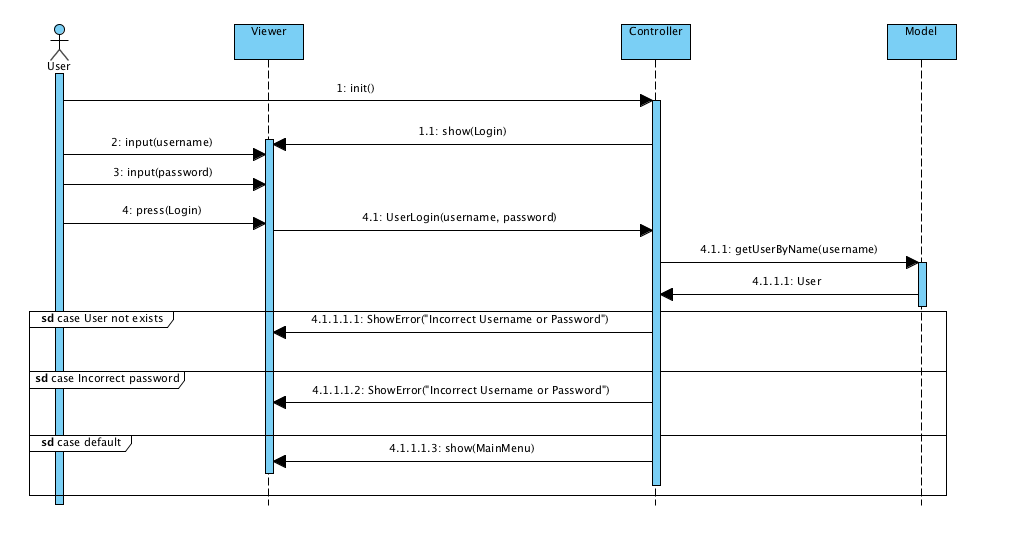
\includegraphics[scale=.5]{SequenceLogin.png}
			\end{center}
		\subsubsection*{Registrieren}
			\begin{center}
				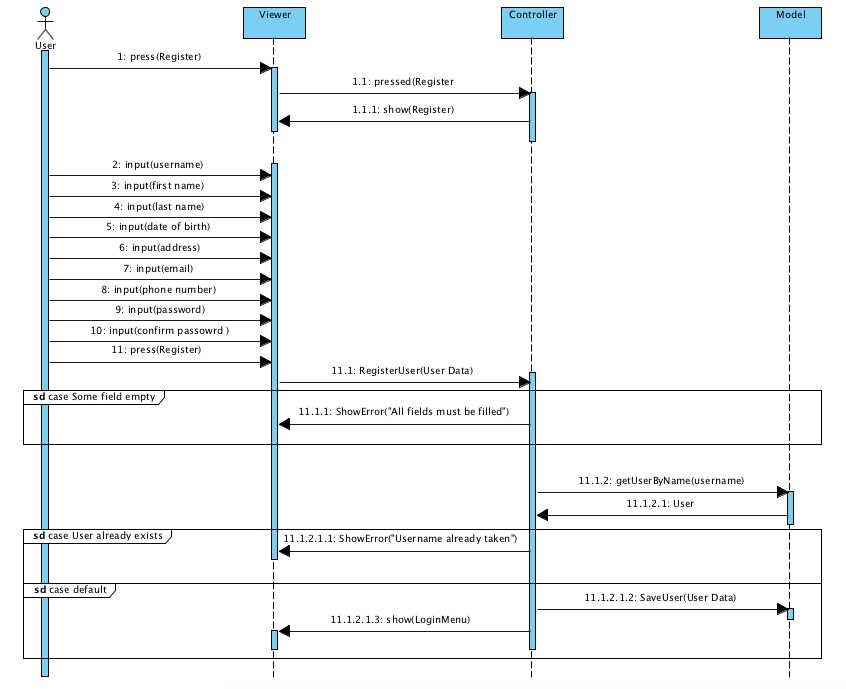
\includegraphics[scale=.5]{SequenceRegister.png}
			\end{center}
		\subsubsection*{Raum erstellen}
			\begin{center}
				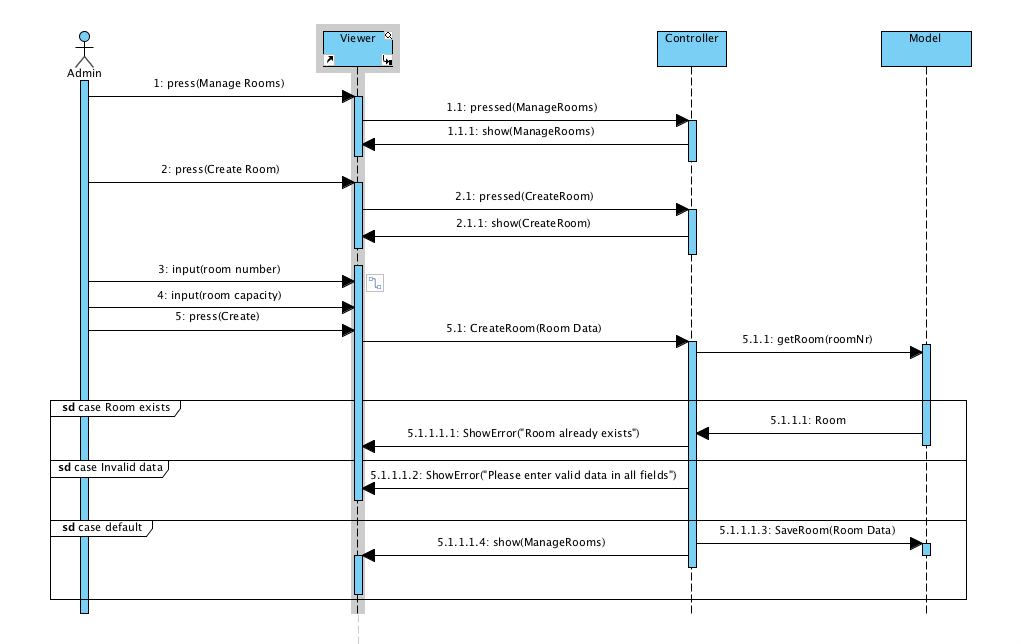
\includegraphics[scale=.5]{SequenceCreateRoom.png}
			\end{center}
	\subsection*{State Machine Diagramme}
		\subsubsection*{Login}
			\begin{center}
				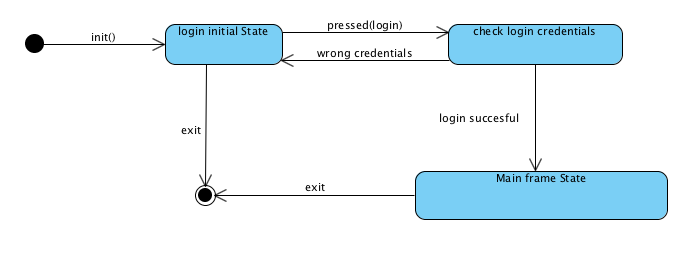
\includegraphics[scale=.5]{sc_login.png}
			\end{center}
		\subsubsection*{Registrieren}
			\begin{center}
				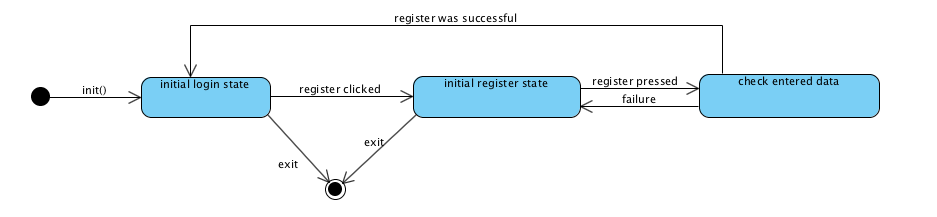
\includegraphics[scale=.5]{sc_register.png}
			\end{center}
		\subsubsection*{Raum erstellen}
			\begin{center}
				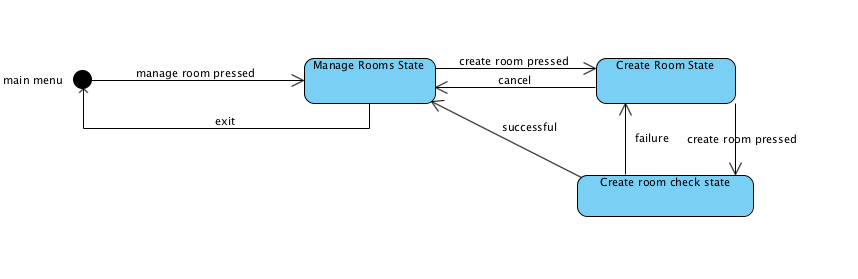
\includegraphics[scale=.5]{sc_manage_room.png}
			\end{center}
\section*{UML Analyse-Klassendiagramm}
\begin{center}
	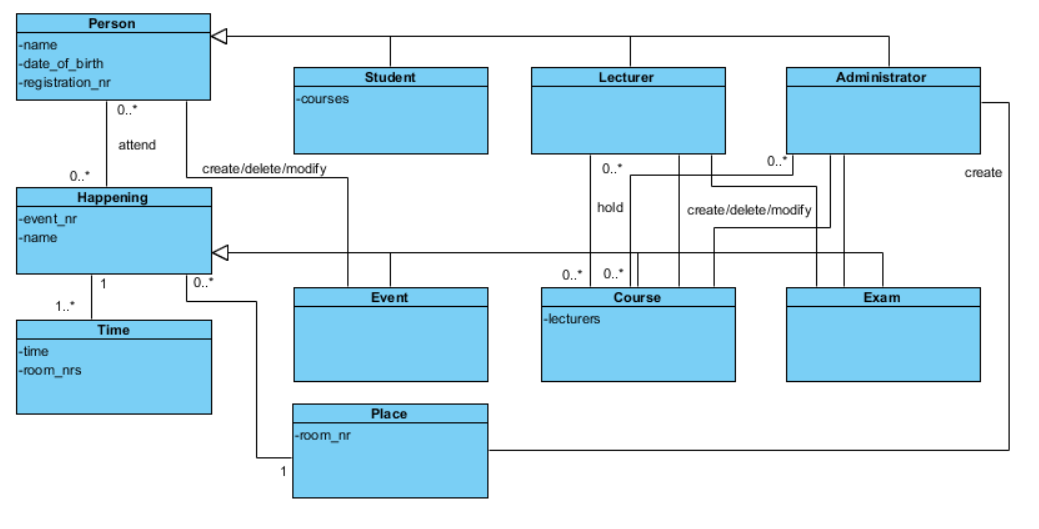
\includegraphics[scale=.7]{AnalysisClassDiagram.png}
\end{center}
\section*{UML Design-Klassendiagramm}
\begin{center}
	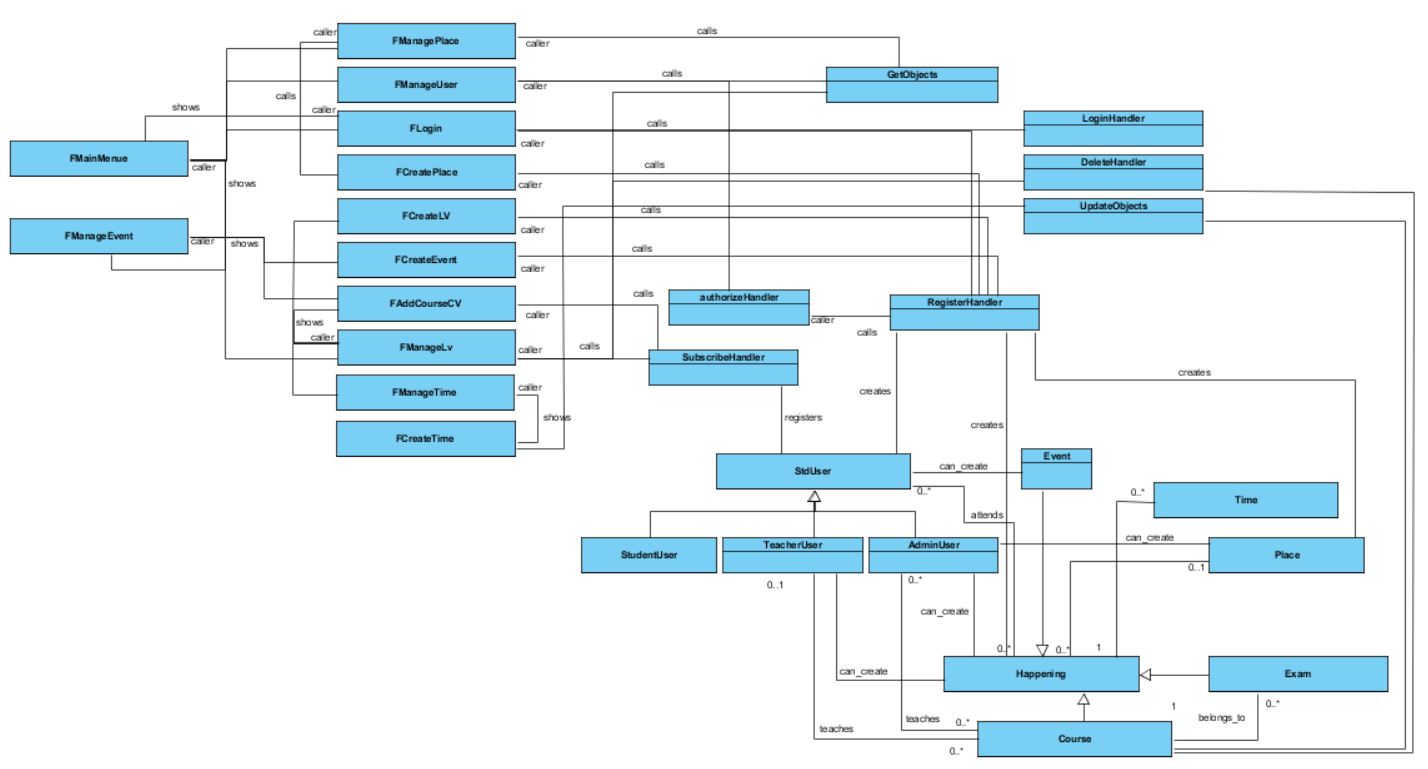
\includegraphics[scale=.5,angle=90]{DesignClassDiagram.png}
\end{center}
\newpage
\section*{Projektplan}
\begin{tabular}{|l|l|}
	\hline
	Accounts erstellen & fertig \\ \hline
	Räume erstellen & fertig \\ \hline
	Veranstaltungen erstellen & fertig \\ \hline
	Veranstaltung suchen & fertig \\ \hline
	Für Veranstaltungen registrieren/abmelden & fertig \\ \hline
	Berechtigungslevel für User & fertig \\ \hline
	Authorisierung von Usern & fertig \\ \hline
	Veranstaltungen suchen & 10.12.2015 \\ \hline
	Manuelle verschiebung von Veranstaltungen & 10.12.2015 \\ \hline
	Zeitplan einsehen & 16.12.2015 \\ \hline
	Automatisches Zeit/Raummanagement & 20.12.2015 \\ \hline
	Zeitpräferenzen für Vortragende & 24.12.2015 \\ \hline
	Semestersystem & 1.1.2016\\ \hline
	Füllung mit endgültigen Daten & 5.1.2016\\ \hline
\end{tabular}
\end{document}